% !TeX root = ../report.tex
\chapter{Grundlagen}\label{chp:theory_of_operation}

Im vorliegenden Bericht wird vielseitig auf praktische Aspekte, die zum Bau eines Passivradars notwendig sind, eingegangen. Um dem Leser das Verständnis dieser Aspekte zu erleichtern, ist es sinnvoll, zunächst die theoretischen Grundlagen zu erläutern. Dieses Kapitel dient der Beschreibung einiger essenzieller Prinzipien, die bei Passivradar zum Einsatz kommen. Dazu wird zunächst der Begriff der bistatischen Geometrie eingeführt und erklärt, anschließend wird diese im Zusammenhang mit passiver Zieldetektion und -lokalisierung kombiniert und mit einer mathematischen Beschreibung versehen. Schließlich wird auf konstruktionsabhängige Eigenarten zur Positionsbestimmung eingegangen.

\section{Bistatische Geometrie}\label{sct:bistatic_geometry}

In der Ortungstechnik versteht man unter dem Begriff der bistatischen Geometrie die räumliche Trennung zwischen einem Sender und einem Empfänger. Bezogen auf Systeme mit mehreren Sendern und Empfängern wird auch der Begriff des multistatischen Systems genutzt. Im umgekehrten Fall, wenn die räumliche Trennung zwischen Sender und Empfänger als vernachlässigbar klein verstanden wird, spricht man von monostatischen Systemen. Die Abbildung~\ref{fig:mono_bi_multistatic_geometry} zeigt vereinfachte Illustrationen dieser Konzepte. Tx und Rx bezeichnen hierbei jeweils Sender und Empfänger im System. Zu beachten hierbei sind die verschiedenen Signalpfade, die sich aus der Anordnung der Sender und Empfänger ergeben. Man unterscheidet zwischen Direkt- und Echosignalen, also jeweils solche die auf direktem Wege von Sender zu Empfänger wandern und solche die erst an einem oder mehreren Objekten reflektieren und dann beim Empfänger eingehen. Letztere werden weiter unterteilt in erwünschte (Ziele, engl.\ Targets) und unerwünschte (engl.\ Clutter) Echos.

\begin{figure}[htb]
    \centering
    \subcaptionbox{Monostatische Geometrie.\label{fig:monostatic_geometry}}{
        \begin{tikzpicture}
            \node at (0,0) [draw,fill=white] (radar) {Tx \& Rx};

            \node [label={above:Ziel}] (target) at (2,2) {\Huge\faPlane};

            \draw [<->,red] (radar) -- (target);
        \end{tikzpicture}
    }
    \subcaptionbox{Bistatische Geometrie.\label{fig:bistatic_geometry}}{
        \begin{tikzpicture}
            \coordinate (rx1_coord) at (-1,0);
            \coordinate (tx1_coord) at (2,0);
            \coordinate (target_coord) at (1.75,1.5);

            \node at (tx1_coord) [draw,fill=white] (tx1) {Tx};
            \node at (rx1_coord) [draw,fill=white] (rx) {Rx};

            \node at (target_coord) [label={above:Ziel}] (target) {\Large\faPlane};

            \draw [->,color=red] (tx1) -- (target);
            \draw [->,color=red] (target) -- (rx);
            \draw [->,color=blue] (tx1) -- (rx);
        \end{tikzpicture}
    }
    \subcaptionbox{Multistatische Geometrie.\label{fig:multistatic_geometry}}{
        \begin{tikzpicture}
            \coordinate (rx1_coord) at (-2,1);
            \coordinate (rx2_coord) at (-1,-0.5);
            \coordinate (tx1_coord) at (3,0);
            \coordinate (tx2_coord) at (2,-1);
            \coordinate (target_coord) at (2,2);

            \node at (tx1_coord) [draw,fill=white] (tx1) {Tx 1};
            \node at (tx2_coord) [draw,fill=white] (tx2) {Tx 2};
            \node at (rx1_coord) [draw,fill=white] (rx1) {Rx 1};
            \node at (rx2_coord) [draw,fill=white] (rx2) {Rx 2};

            \node at (target_coord) [label={above:Ziel}] (target) {\Large\faPlane};

            \draw [->,color=red] (tx1) -- (target);
            \draw [->,color=red] (tx2) -- (target);
            \draw [->,color=red] (target) -- (rx1);
            \draw [->,color=red] (target) -- (rx2);
            \draw [->,color=blue] (tx1) -- (rx1);
            \draw [->,color=blue] (tx1) -- (rx2);
            \draw [->,color=blue] (tx2) -- (rx1);
            \draw [->,color=blue] (tx2) -- (rx2);
        \end{tikzpicture}
    }

    \caption{Mono-, Bi- und Multistatische Geometrie.}\label{fig:mono_bi_multistatic_geometry}
\end{figure}

Ein weiterer wichtiger Begriff im Zusammenhang mit bistatischer Geometrie ist die bistatische Entfernung. Malanowski definiert diese in~\cite[S.~10]{Malanowski2019} wie folgt:

\begin{equation}
    R = R_1 + R_2 - R_\text{b}
\end{equation}\label{eq:bistatic_range}

Wobei \(R_\text{b}\) die Strecke des Direktpfades bezeichnet. Die Terme \(R_1\) und \(R_2\) bezeichnen jeweils die Strecke vom Sender zum Ziel und vom Ziel zum Empfänger. Zusammen wird \(R_1 + R_2\) auch als bistatische Summe bezeichnet. Bildlich gesprochen versteht man unter bistatischer Entfernung die zusätzliche Strecke, die das Echosignal gegenüber dem Direktsignal zurückgelegt hat. Abbildung~\ref{fig:bistatic_range} zeigt diesen Zusammenhang grafisch. Gezeigt ist neben den genannten Größen auch ein Geschwindigkeitsvektor \(\boldsymbol{v}\) des Ziels, sowie der s.\,g.\@ bistatische Winkel \(\beta \), definiert zwischen den Sichtlinien von Sender und Empfänger am Ziel. Der Term \(\delta \) bezeichnet den Winkel zwischen der Winkelhalbierenden von \(\beta \) und \(\boldsymbol{v}\).

\begin{figure}[htb]
    \begin{minipage}[b]{0.49\linewidth}
        \centering
        \begin{tikzpicture}
            \coordinate (rx1_coord) at (-2,0);
            \coordinate (tx1_coord) at (2,0);
            \coordinate (target_coord) at (1.75,2.5);
            \coordinate (v_vec) at (2,0);

            \node at (tx1_coord) [draw,fill=white] (tx1) {Tx};
            \node at (rx1_coord) [draw,fill=white] (rx) {Rx};

            \node at (target_coord) [label={above:Ziel}] (target) {\Large\faPlane};

            \draw [->,color=red] (tx1) -- (target) node [black,midway,right] {$R_1$};
            \draw [->,color=red] (target) -- (rx) node [black,midway,above left] {$R_2$};
            \draw [->,color=blue] (tx1) -- (rx) node [black,midway,below] {$R_\text{b}$};

            \pic [draw,angle radius=0.8cm,angle eccentricity=0.8,"\contour{white}{$\beta$}"] {angle=rx1_coord--target_coord--tx1_coord};

            \draw [dotted] let
            \p1 = ($(target_coord)!1cm!(rx1_coord)$),
            \p2 = ($(target_coord)!1cm!(tx1_coord)$),
            \p3 = ($(\p1) + (\p2) - (target_coord)$)
            in
            ($(target_coord)!1!(\p3)$) coordinate (A) -- ($(\p3)!1!(target_coord)$);

            \path let \p1=($(target_coord)+(v_vec)$) in
            (rx1_coord) -- (target_coord) coordinate (B) -- (\p1) coordinate (C) pic [draw,angle radius=1.1cm,angle eccentricity=0.8,"\contour{white}{$\delta$}"] {angle};

            \draw let \p1=($(target_coord)+(v_vec)$) in [->,color=cyan] (target) -- node [black,midway,above,align=center] {$\boldsymbol{v}$} (\p1);
        \end{tikzpicture}
        \subcaption{Bistatische Geometrie.\label{fig:bistatic_range_model}}
    \end{minipage}
    \begin{minipage}[b]{0.49\linewidth}
        \centering
        \begin{tikzpicture}
            \coordinate (rx1_coord) at (-2,0);
            \coordinate (tx1_coord) at (2,0);
            \coordinate (target_coord) at (1.75,2);

            \draw [dotted,color=gray]
            let
            \p1=($(tx1_coord)-(target_coord)$),
            \p2=($(target_coord)-(rx1_coord)$),
            \p3=($(tx1_coord)-(rx1_coord)$),
            \n1={veclen(\x1,\y1)},
            \n2={\n1+veclen(\x2,\y2)},
            \n3={\n2-veclen(\x3,\y3)}
            in
            (\n1,0) edge node [black,midway,right,align=center] {$+$} (\n1,-1)
            (\n2,-1) edge node [black,midway,right,align=center] {$-$} (\n2,-2)
            (\n3,-2) edge node [black,midway,right,align=center] {$=$} (\n3,-3);

            \draw [->,color=red]
            let
            \p1=($(tx1_coord)-(target_coord)$),
            \n1={veclen(\x1,\y1)}
            in
            (0,0) -- node [black,midway,above,align=center] {$R_1$} (\n1,0);
            \draw [->,color=red]
            let
            \p1=($(tx1_coord)-(target_coord)$),
            \p2=($(target_coord)-(rx1_coord)$),
            \n1={veclen(\x1,\y1)},
            \n2={\n1+veclen(\x2,\y2)}
            in
            (\n1,-1) -- node [black,midway,above,align=center] {$R_2$} (\n2,-1);
            \draw [->,color=blue]
            let
            \p1=($(tx1_coord)-(target_coord)$),
            \p2=($(target_coord)-(rx1_coord)$),
            \p3=($(tx1_coord)-(rx1_coord)$),
            \n1={veclen(\x1,\y1)},
            \n2={\n1+veclen(\x2,\y2)},
            \n3={\n2-veclen(\x3,\y3)}
            in
            (\n2,-2) -- node [black,midway,above,align=center] {$R_{\text{b}}$} (\n3,-2);

            \draw [->,color=green]
            let
            \p1=($(tx1_coord)-(target_coord)$),
            \p2=($(target_coord)-(rx1_coord)$),
            \p3=($(tx1_coord)-(rx1_coord)$),
            \n1={veclen(\x1,\y1)},
            \n2={\n1+veclen(\x2,\y2)},
            \n3={\n2-veclen(\x3,\y3)}
            in
            (0,-3) -- node [black,midway,above,align=center] {$R$} (\n3,-3);
        \end{tikzpicture}
        \subcaption{Bistatische Entfernung.\label{fig:bistatic_range_equation}}
    \end{minipage}
    \caption{Grafische Herleitung der bistatischen Entfernung.}\label{fig:bistatic_range}
\end{figure}

Weitere Einsicht bietet die kartesische Betrachtung der bistatischen Entfernung. Ausgehend vom zweidimensionalen Fall werden zunächst Sender, Empfänger und Ziel kartesischen Koordinaten zugewiesen. Es gelten für die Position des Senders \(\boldsymbol{p}_\text{tx} = \begin{bmatrix} x_\text{tx}, y_\text{tx} \end{bmatrix}\), für die Position des Empfängers \(\boldsymbol{p}_\text{rx} = \begin{bmatrix} x_\text{rx}, y_\text{rx} \end{bmatrix}\) und die Position des Ziels \(\boldsymbol{p} = \begin{bmatrix} x, y \end{bmatrix}\). Dafür ergibt sich für die Entfernungen

\begin{equation}
    R_1 = {\lVert \boldsymbol{p} - \boldsymbol{p}_\text{tx} \rVert}_2 = \sqrt{{(x - x_\text{tx})}^2 + {(y - y_\text{tx})}^2}
\end{equation}
\begin{equation}
    R_2 = {\lVert \boldsymbol{p} - \boldsymbol{p}_\text{rx} \rVert}_2 = \sqrt{{(x - x_\text{rx})}^2 + {(y - y_\text{rx})}^2}
\end{equation}
\begin{equation}
    R_\text{b} = {\lVert \boldsymbol{p_\text{tx}} - \boldsymbol{p}_\text{rx} \rVert}_2 = \sqrt{{(x_\text{tx} - x_\text{rx})}^2 + {(y_\text{tx} - y_\text{rx})}^2}
\end{equation}

Eingesetzt in die ursprüngliche Gleichung~\ref{eq:bistatic_range}, beschreiben diese Gleichungen eine Ellipse, deren Lösungsmenge die möglichen Positionen des Ziels für eine gegeben bistatische Entfernung darstellt. Die Konstruktion dieser Ellipse ist in Abbildung~\ref{fig:bistatic_ellipse} illustriert. Position des Senders und Empfängers bilden jeweils die Brennpunkte der Ellipse. Der Term \(R_\text{b}\) wird für den Zeitraum der Messung als bekannt vorausgesetzt. Die Summe der beiden Terme \(R_1\) und \(R_2\) ist durch Messung der bistatische Entfernung \(R\) beschränkt. Durch Variation von \(R_1\) und \(R_2\) ergibt sich eine Ellipsenform. Diese wird in der Literatur auch als bistatische Ellipse bezeichnet.

\begin{figure}[htb]
    \centering
    \begin{tikzpicture}
        \def\F{5}
        \coordinate (rx1_coord) at (-\F,0);
        \coordinate (tx1_coord) at (\F,0);
        \coordinate (target_coord) at (2,3.5);
        \coordinate (pencil) at (0.1,0.6);

        \draw (0,0)
        let
        \p1=($(target_coord)-(tx1_coord)$),
        \p2=($(target_coord)-(rx1_coord)$),
        \p3=(tx1_coord),
        \n1={scalar((veclen(\x1,\y1) + veclen(\x2,\y2))*1pt/1cm)},
        \n2={sqrt(pow(\n1/2, 2))},
        \n3={sqrt(pow(\n1/2, 2) - pow(\F, 2))}
        in
        circle [x radius=\n2,y radius=\n3,draw=gray];

        \draw [dotted] (rx1_coord) node [cross out,draw,solid] {} node [below=0.1cm] {Rx} -- (0,0) node {\contour{white}{$R_{\text{b}}$}} -- (tx1_coord) node [cross out,draw,solid] {} node [below=0.1cm] {Tx};

        \draw [dash dot] (rx1_coord) -- (target_coord) node [midway] {\contour{white}{$R_{2}$}} -- (tx1_coord) node [midway] {\contour{white}{$R_{1}$}};

        \draw [<-] (target_coord) -- ++(pencil);

        \node at (0,-1.5) {%
            \(\begin{aligned}
                    & R_{1} + R_{2}                & = \text{const.} & \dots \text{bistatische Summe}      \\
                R = & R_{1} + R_{2} - R_{\text{b}} & = \text{const.} & \dots \text{bistatische Entfernung} \\
            \end{aligned}
            \)};
    \end{tikzpicture}
    \caption{Schematische Darstellung der bistatischen Ellipsoidengleichung.}\label{fig:bistatic_ellipse}
\end{figure}

Eine Erweiterung auf den dreidimensionalen Fall ergibt statt einer Ellipse einen Ellipsoiden, auch bistatischer Ellipsoid genannt. Abbildung~\ref{fig:bistatic_ellipsoid} zeigt exemplarisch einen solchen bistatischen Ellipsoid. Die Lösungen der Ellipsoidengleichung bilden die möglichen Positionen des Ziels für eine gegebene bistatische Entfernung. Eine genauere Modellierung der kartesischen Position wird in~\cite{Willis2005} vorgenommen.

\begin{figure}[htb]
    \centering
    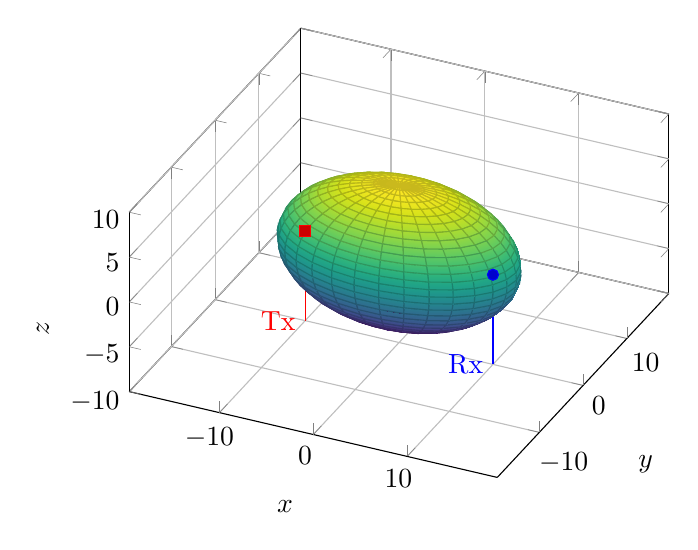
\begin{tikzpicture}
        \def\R{25}
        \def\F{10}
        \def\a{sqrt((\R/2)^2)}
        \def\b{sqrt((\R/2)^2 - \F^2)}
        \def\c{\b}
        \def\xmin{-int(\a + 5 - mod(\a - 5, 5))}
        \def\ymin{-int(\b + 5 - mod(\b - 5, 5))}
        \def\zmin{-int(\c + 5 - mod(\c - 5, 5))}
        \def\xmax{+int(\a + 5 - mod(\a - 5, 5))}
        \def\ymax{+int(\b + 5 - mod(\b - 5, 5))}
        \def\zmax{+int(\c + 5 - mod(\c - 5, 5)))}
        \begin{axis}[
                z buffer=sort,
                axis equal,
                colormap/viridis,
                samples=31,
                xmin=\xmin,
                ymin=\ymin,
                zmin=\zmin,
                xmax=\xmax,
                ymax=\ymax,
                zmax=\zmax,
                xlabel=$x$,
                ylabel=$y$,
                zlabel=$z$,
                grid=major,
                view/az=25,
                view/el=30,
            ]
            \addplot3 coordinates {
                    (\F,0,0)
                    (\F,0,\zmin)
                } node[left,pos=0] {Rx};
            \addplot3 coordinates {
                    (-\F,0,0)
                    (-\F,0,\zmin)
                } node[left,pos=0] {Tx};
            \addplot3 [
                surf,
                shader=faceted interp,
                opacity=1,
                domain=0:180,
                y domain=0:360,
            ] (
            {\a*sin(x)*cos(y)},
            {\b*sin(x)*sin(y)},
            {\c*cos(x)}
            );
        \end{axis}
    \end{tikzpicture}
    \caption{Exemplarischer bistatischer Ellipsoid für \(R = 15\) und \(R_\text{b} = 10\).}\label{fig:bistatic_ellipsoid}
\end{figure}

Eine weitere messbare Eigenschaft des Echosignals ist der Dopplereffekt relativ zum Referenzsignal. Unter Annahme stationärer Sender und Empfänger erlaubt dies die Bestimmung der s.\,g.\@ bistatischen Geschwindigkeit. Im allgemeinen Fall (auch in solchen in denen die eben getroffene Annahme nicht zutrifft), bildet die bistatische Geschwindigkeit die erste Ableitung der bistatischen Summe; geometrisch betrachtet also die Rate der Vergrößerung oder Verkleinerung der bistatischen Ellipse (bzw. Ellipsoiden) über die Zeit~\cite[S.~119]{Willis2005}. Über diese simple geometrische Darstellung lassen sich recht einfach die Gradienten maximaler und minimaler bistatischer Geschwindigkeit finden, gezeigt in Abbildung~\ref{fig:bistatic_velocity}. Dabei ist festzustellen, dass die Gradienten maximaler bistatischer Geschwindigkeit stets entlang dem Winkelhalbierenden Vektor von \(\beta \) aus Abbildung~\ref{fig:bistatic_range_model} verlaufen. Folgt man den Gradienten zu jedem Zeitschritt, ergeben sich Hyperbeln konstanter bistatischer Geschwindigkeit.

\begin{figure}[htb]
    \centering
    \begin{tikzpicture}
        \def\F{5}
        \coordinate (l_foci_coord) at (-\F,0);
        \coordinate (r_foci_coord) at (\F,0);
        \coordinate (point_on_ellipse_coord) at (6,0);

        \draw (0,0)
        let
        \p1=($(point_on_ellipse_coord)-(r_foci_coord)$),
        \p2=($(point_on_ellipse_coord)-(l_foci_coord)$),
        \n1={scalar((veclen(\x1,\y1) + veclen(\x2,\y2))*1pt/1cm)},
        \n2={\n1/2},
        \n3={sqrt(pow(\n1/2, 2) - pow(\F, 2))}
        in
        circle [x radius=\n2,y radius=\n3,draw=gray];

        \draw [dotted] (l_foci_coord) node [cross out,draw,solid] {} -- (0,0) node {\contour{\thepagecolor}{$R_{\text{b}}$}} -- (r_foci_coord) node [cross out,draw,solid] {};

        \foreach \u in {-5.5,-5,...,5.5} {
                \draw [->,blue] let
                \p1=($(point_on_ellipse_coord)-(r_foci_coord)$),
                \p2=($(point_on_ellipse_coord)-(l_foci_coord)$),
                \n1={scalar((veclen(\x1,\y1) + veclen(\x2,\y2))*1pt/1cm)},
                \p3=(\u,{sqrt( (pow(2 * \F / \n1, 2) - 1) * pow(\u, 2) + pow(\n1 / 2, 2) - pow(\F, 2) )}),
                \p4=($(\p3)!1cm!(l_foci_coord)$),
                \p5=($(\p3)!1cm!(r_foci_coord)$),
                \p6=($(\p4) + (\p5) - (\p3)$),
                in
                (\p3) -- ($(\p6)!1.5!(\p3)$);
            }

        \foreach \u in {-6,6} {
                \draw [->,blue] let
                \p1=(\u,0),
                \p2=($(\p1)!1cm!(l_foci_coord)$),
                \p3=($(\p1)!1cm!(r_foci_coord)$),
                \p4=($(\p2) + (\p3) - (\p1)$),
                in
                (\p1) -- ($(\p4)!1.5!(\p1)$);
            }

        \foreach \u in {-5.5,-5,...,5.5} {
                \draw [->,blue] let
                \p1=($(point_on_ellipse_coord)-(r_foci_coord)$),
                \p2=($(point_on_ellipse_coord)-(l_foci_coord)$),
                \n1={scalar((veclen(\x1,\y1) + veclen(\x2,\y2))*1pt/1cm)},
                \p3=(\u,{-sqrt( (pow(2 * \F / \n1, 2) - 1) * pow(\u, 2) + pow(\n1 / 2, 2) - pow(\F, 2) )}),
                \p4=($(\p3)!1cm!(l_foci_coord)$),
                \p5=($(\p3)!1cm!(r_foci_coord)$),
                \p6=($(\p4) + (\p5) - (\p3)$),
                in
                (\p3) -- ($(\p6)!1.5!(\p3)$);
            }
    \end{tikzpicture}
    \caption{Gradienten maximaler positiver bistatischer Geschwindigkeit.}\label{fig:bistatic_velocity}
\end{figure}

\section{Passive Zieldetektion und -lokalisierung}

Wie die verwendung des Akronyms Passiv\emph{radar} (\textbf{Ra}dio %
% cspell:disable-next-line
\textbf{D}etection %
\textbf{a}nd \textbf{R}anging) bereits vermuten lässt, handelt es sich bei den Ausstrahlungen der Sender um elektromagnetische Wellen im Radio oder Mikrowellenbereich. Sender werden in der Literatur auch Beleuchter oder Illuminator bezeichnet. Diese werden anders als bei aktivem Radar nicht vom Operator selbst gesteuert. Stattdessen dienen sie oft einer ganz anderen Primärfunktion, wie bspw.\ Hör-, Mobilfunk oder Fernsehen. Die vorliegenden Wellenformen können somit unvorteilhafte Eigenschaften in Bezug auf Radar aufweisen.

Aufgrund der Nutzung von Beleuchtern aus der Umgebung ist grundsätzlich von einer bistatischen Systemanordnung wie in Abschnitt~\ref{sct:bistatic_geometry} auszugehen. Die zur Ziellokalisierung genutzte Messgröße ist dabei stets der gemessene Zeitversatz \(\tau \) zwischen Echo- und Direktsignal. Die genaue Bestimmung des Zeitversatzes geschieht i.\,d.\,R. mittels Kreuzambiguitätsfunktion, diese wird näher in Abschnitt~\ref{sct:ambiguity_function} erklärt. Wie in Gleichung~\ref{eq:bistatic_delay_measurement} ergibt sich daraus unter Berücksichtigung der Ausbreitungsgeschwindigkeit elektromagnetischer Wellen \(c \approx 3\cdot10^8\) direkt die bistatische Entfernung \(R\)~\cite[S.~11]{Malanowski2019}.

\begin{equation}
    R = c \cdot \tau
\end{equation}\label{eq:bistatic_delay_measurement}

Dabei ist festzustellen, dass ohne zusätzliche Informationen keine Rückschlüsse auf die kartesische Position des Ziels getroffen werden können. Hierzu ist entweder die Zuhilfenahme mehrerer Messungen der bistatischer Entfernung oder, sofern die Bauart des Systems es erlaubt, der Winkel des eintreffenden Echos notwendig. Abbildung~\ref{fig:localization_via_multiple_bistatic_ranges} zeigt wie eine Ziellokalisierung mittels mehrerer bistatischer Entfernungsmessungen ausgehend von drei Beleuchtern ablaufen kann. Hierbei ist festzuhalten, dass zur Ermittlung einer eindeutigen Position im zweidimensionalen Fall drei Ellipsenschnitte notwendig sind. Im dreidimensionalen erhöht sich dies auf vier Ellipsoidenschnitte. Bei nur drei oder weniger Ellipsoiden entstehen Schnittmengen mit zwei oder mehr Positionen, hier kann die Schnittmenge unter Anwendung geometrischer Einschränkungen oft reduziert werden (z.\,B. bei Lösungen unter Terrainhöhe können Flugzeuge ausgeschlossen werden). An bis zu dieser Stelle würde außerdem kein Messrauschen beachtet. In der Realität kann es somit auch vorkommen, dass bei ausreichend Beleuchtern dennoch keine eindeutige Lösung gefunden werden kann. Abbildung~\ref{fig:localization_via_angular_measurement} zeigt wie die Lokalisierung über Winkelmessung erfolgt. Dazu kommen oft Antennenarrays mit digital steuerbarer Hauptkeule zum Einsatz, welche eine schnelle Abtastung des Ellipsoiden erlauben. Die Positionsgenauigkeit ist hierbei in direkter Abhängigkeit von der Breite der Antennenhauptkeule und damit der Winkelauflösung des Antennenarrays.

\begin{figure}[htb]
    \centering
    \begin{tikzpicture}

        \coordinate (rx1_coord) at (-5,0);
        \coordinate (tx1_coord) at (5,0);
        \coordinate (tx2_coord) at (2,2);
        \coordinate (tx3_coord) at (6,-3);
        \coordinate (target_coord) at (-2,-3.5);

        \draw [red]
        let
        \p1=(tx1_coord),
        \p2=($(target_coord)-(\p1)$),
        \p3=($(target_coord)-(rx1_coord)$),
        \p4=($(\p1)-(rx1_coord)$),
        \n1={scalar((veclen(\x2,\y2) + veclen(\x3,\y3))*1pt/1cm)},
        \n2={scalar(veclen(\x4,\y4)*1pt/1cm)},
        \n3={sqrt(pow(\n1/2, 2))},
        \n4={sqrt(pow(\n1/2, 2) - pow(\n2/2, 2))},
        in
        ($(rx1_coord)!0.5!(\p1)$)
        circle [x radius=\n3,y radius=\n4,draw=gray];

        \draw [green]
        let
        \p1=(tx2_coord),
        \p2=($(target_coord)-(\p1)$),
        \p3=($(target_coord)-(rx1_coord)$),
        \p4=($(\p1)-(rx1_coord)$),
        \p5=(rx1_coord),
        \n1={scalar((veclen(\x2,\y2) + veclen(\x3,\y3))*1pt/1cm)},
        \n2={scalar(veclen(\x4,\y4)*1pt/1cm)},
        \n3={sqrt(pow(\n1/2, 2))},
        \n4={sqrt(pow(\n1/2, 2) - pow(\n2/2, 2))},
        \n5={atan2(scalar(\y1*1pt/1cm),scalar(\x1*1pt/1cm)-scalar(\x5*1pt/1cm))},
        in
        ($(rx1_coord)!0.5!(\p1)$)
        circle [x radius=\n3,y radius=\n4,draw=gray,rotate=\n5];

        \draw [blue]
        let
        \p1=(tx3_coord),
        \p2=($(target_coord)-(\p1)$),
        \p3=($(target_coord)-(rx1_coord)$),
        \p4=($(\p1)-(rx1_coord)$),
        \p5=(rx1_coord),
        \n1={scalar((veclen(\x2,\y2) + veclen(\x3,\y3))*1pt/1cm)},
        \n2={scalar(veclen(\x4,\y4)*1pt/1cm)},
        \n3={sqrt(pow(\n1/2, 2))},
        \n4={sqrt(pow(\n1/2, 2) - pow(\n2/2, 2))},
        \n5={atan2(scalar(\y1*1pt/1cm),scalar(\x1*1pt/1cm)-scalar(\x5*1pt/1cm))},
        in
        ($(rx1_coord)!0.5!(\p1)$)
        circle [x radius=\n3,y radius=\n4,draw=gray,rotate=\n5];

        \draw [dotted,red] (rx1_coord) -- (tx1_coord) node [cross out,draw,solid] {} node [below=2pt] {Tx1};
        \draw [dotted,green] (rx1_coord) -- (tx2_coord) node [cross out,draw,solid] {} node [below=2pt] {Tx2};
        \draw [dotted,blue] (rx1_coord) -- (tx3_coord) node [cross out,draw,solid] {} node [below=2pt] {Tx3};

        \node at (target_coord) {\huge\faPlane};
        \path (rx1_coord) node [below=2pt] {Rx} node [cross out,draw,solid] {};
    \end{tikzpicture}
    \caption{Ziellokalisierung über Messung mehrerer bistatischer Entfernungen in einem System mit drei Sendern.}\label{fig:localization_via_multiple_bistatic_ranges}
\end{figure}

\begin{figure}[htb]
    \centering
    \begin{tikzpicture}
        \coordinate (rx1_coord) at (-5,0);
        \coordinate (tx1_coord) at (5,0);
        \coordinate (target_coord) at (-2,-3.5);
        \coordinate (horizon) at (0,0);

        \begin{scope}
            \clip
            let
            \p1=(tx1_coord),
            \p2=($(target_coord)-(\p1)$),
            \p3=($(target_coord)-(rx1_coord)$),
            \p4=($(\p1)-(rx1_coord)$),
            \n1={scalar((veclen(\x2,\y2) + veclen(\x3,\y3))*1pt/1cm)},
            \n2={scalar(veclen(\x4,\y4)*1pt/1cm)},
            \n3={sqrt(pow(\n1/2, 2))},
            \n4={sqrt(pow(\n1/2, 2) - pow(\n2/2, 2))},
            in
            ($(rx1_coord)!0.5!(\p1)$)
            circle [x radius=\n3,y radius=\n4];

            \foreach \angle in {-50} {
                    \path [rotate around={{\angle+5}:(rx1_coord)}]
                    let
                    \p1=(tx1_coord),
                    \p2=($(target_coord)-(\p1)$),
                    \p3=($(target_coord)-(rx1_coord)$),
                    \n1={scalar((veclen(\x2,\y2) + veclen(\x3,\y3))*1pt/1cm)},
                    \n3={sqrt(pow(\n1/2, 2)) + 1},
                    in
                    (rx1_coord) -- (\n3,0) node (a) {};
                    \path [rotate around={{\angle-5}:(rx1_coord)}]
                    let
                    \p1=(tx1_coord),
                    \p2=($(target_coord)-(\p1)$),
                    \p3=($(target_coord)-(rx1_coord)$),
                    \n1={scalar((veclen(\x2,\y2) + veclen(\x3,\y3))*1pt/1cm)},
                    \n3={sqrt(pow(\n1/2, 2)) + 1},
                    in
                    (rx1_coord) -- (\n3,0) node (b) {};

                    \fill [red,opacity=0.5] (rx1_coord) -- (a.center) -- (b.center);
                }
        \end{scope}
        \draw [dotted] (rx1_coord) -- (horizon);

        \pic [draw,angle radius=1cm,angle eccentricity=0.8,"\(\alpha \)"] {angle=target_coord--rx1_coord--horizon};

        \node (antenna_north) [above=0.4 of rx1_coord,anchor=south] {};
        \node (antenna_east) [base right=0.4 of rx1_coord,anchor=south] {};
        \node (antenna_south) [below=0.4 of rx1_coord,anchor=south] {};
        \node (antenna_west) [base left=0.4 of rx1_coord,anchor=south] {};

        \node [bareantenna,scale=0.5,above=0 of antenna_north.south] {};
        \node [bareantenna,scale=0.5,above=0 of antenna_east.south] {};
        \node [bareantenna,scale=0.5,above=0 of antenna_south.south] {};
        \node [bareantenna,scale=0.5,above=0 of antenna_west.south] {};

        \draw (antenna_north.south) -- (rx1_coord) edge (antenna_east.south) -- (rx1_coord) edge (antenna_south.south) -- (rx1_coord) edge (antenna_west.south) -- (rx1_coord);

        \draw
        let
        \p1=(tx1_coord),
        \p2=($(target_coord)-(\p1)$),
        \p3=($(target_coord)-(rx1_coord)$),
        \p4=($(\p1)-(rx1_coord)$),
        \n1={scalar((veclen(\x2,\y2) + veclen(\x3,\y3))*1pt/1cm)},
        \n2={scalar(veclen(\x4,\y4)*1pt/1cm)},
        \n3={sqrt(pow(\n1/2, 2))},
        \n4={sqrt(pow(\n1/2, 2) - pow(\n2/2, 2))},
        in
        ($(rx1_coord)!0.5!(\p1)$)
        circle [x radius=\n3,y radius=\n4,draw=gray];

        \node at (target_coord) {\huge\faPlane};
    \end{tikzpicture}
    \caption{Ziellokalisierung über bistatische Entfernung und Winkelmessung.}\label{fig:localization_via_angular_measurement}
\end{figure}

Die bistatische Geschwindigkeit \(V\) lässt sich über die gemessene Dopplerfrequenz \(f_{\text{d}} = f - f_{0}\) und Wellenlänge des Signals \(\lambda = c / f_{c}\) wie folgt bestimmen~\cite[S.~12]{Malanowski2019}:

\begin{equation}\label{equ:bistatic_velocity}
    V = -\lambda \cdot f_{\text{d}}
\end{equation}

Sie kann unter anderem zur Initialisierung von bistatischen Tracks genutzt werden~\cite{Petsios2007}, spielt aber auch eine essenzielle Rolle in der Unterdrückung von statischem Clutter und dem herausfiltern potenziell relevanter Ziele.
